\section{TCP: Principles and practice}
\subsection{TCP headers}
\textbf{Part 1}\\
\begin{enumerate}
\item The purpose of the RST bit is to reset a connection. It is used
  when a client (or server) sends an invalid TCP segment. If for instance a
  client sends a SYN, receives a SYN-ACK, and then sends another SYN, the server
  will most likely send a RST packet.
\item The sequence number is sent with each segment of data. The first octet in
  the segment has a sequence number, which represents the segments sequence
  number. The acknowledgment number is part of the sequence number, and is used
  to identify the next expected octet.\\
  There is a relation between the sender and the receiver, otherwise the data
  sent could be arbitrary rubble.
\item The TCP window is used to indicate how much data the receiver is
  ready/willing to receive from the sender. A positive window size tells how
  many bytes the receivers buffer is able to hold.
\item The sender starts a timer and waits a certain amount of time, before
  sending a new package. The ACK from the receiver to the sender, should then
  contain a new window size, which is able to hold the data that the sender
  wants to send.
\end{enumerate}

\noindent \textbf{Part 2}
The client is able to send data to the server after receiving the sequence and
acknowledgment numbers with the SYN-ACK packet.\\

\noindent \textbf{Part 3}
\begin{wrapfigure}{L}{1\textwidth}
  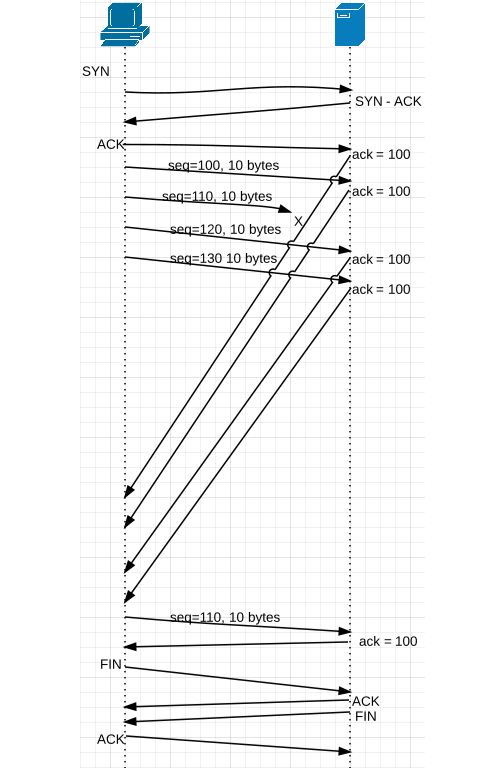
\includegraphics[scale=0.5]{tcpstuff.png}
\end{wrapfigure}

